\chapter{Distributed AEP}

\section{Self-learning Autonomous Edge Learning and Inferencing Pipeline (AEP)}
\label{AEP}
The Autonomous Edge Learning and Inferencing Pipeline (AEP) is an innovative approach designed to harness the potential of unsupervised learning in IoT environments. At its core, the AEP consists of two main stages:
\begin{enumerate}
    \item Pseudo-label Generation, using the k-means++ clustering technique, intelligently groups unlabeled data.
    \item Local Training and Classification, where once pseudo-labels are assigned, the AEP engages in the training process with either the decision tree (DT) or the k-nearest neighbor (k-NN) classifiers.
\end{enumerate}

This system stands out particularly for its adaptability in resource-constrained scenarios, ensuring efficient on-device ML operations. The creation of AEP comes in response to the challenge of managing vast amounts of unlabeled data generated by IoT devices, pushing the boundaries of traditional supervised learning models. Its design prioritizes flexibility and robustness, making it suitable for various microcontrollers and edge devices. It achieves robustness thanks to its sample filtering, used to delete outliers. Moreover, it can cope with the constant inflow of data with memory overflow control techniques, using FIFO, RND, and CONF memory filtering. FIFO (First In First Out) prioritizes new data over old data. When the memory is full, the oldest samples are deleted to accommodate the newest ones. RND, instead, randomly selects some samples to delete. CONF selects the data points to delete based on their confidence level. The confidence level measures how likely a data point is valuable. Euclidean distance measures how close the sample is to the kmeans++ centroids. There are also three parameters for the memory management of the pipeline. The memory size indicates how many samples we want to be saved at any time. The initial threshold and the update threshold are used to decide how the pipeline behaves. The initial threshold is the starting memory size, which is then increased by increments of magnitude update threshold until reaching the memory size. When the memory is full, the incoming data are accepted by freeing memory with the methodologies stated above. In the paper, there are also efficiency tests and many considerations on memory and CPU usage. I will not delve into such details since I only use the AEP as a starting point for my DML approach. I have modified the AEP to better fit the goal of distributing it albeit preserving its memory-constrained and power-efficiency characteristics. How I modified it and why will be discussed in the Distributed AEP chapter.
% Remember to add the ref to the paper


\label{cha:distributed_aep}
The primary objective of this study was to decentralize the autonomous edge learning and inferencing pipeline (AEP), across a network of low-power nodes. The challenge lies in enhancing the inference accuracy without incurring significant data communication overheads or computational burdens. The starting point for this endeavor was an existing AEP, the source code for which was publicly accessible on GitHub; readers can find the repository link within the associated paper. The subsequent sections detail the modifications made to tailor the pipeline to the outlined scenario, followed by an overview of simulation processes implemented in Python. The final implementation, encompassing the system design and algorithm for node contribution aggregation, was not without its challenges, discussed comprehensively in the System Implementation section. For verification purposes, one of the two datasets used by the original AEP creators was employed, specifically the Pima Indians Diabetes Database\cite{diabetes_db}, intended for diabetes detection. The second dataset, related to semiconductor manufacturing process anomalies, was not chosen due to its already high inference accuracy achieved by the original AEP. With the Pima database, the initial accuracy was approximately 70\%, offering potential avenues for enhancement.

% Add reference to database

\section{AEP Modification}
\label{sec:aep_modification}

The AEP required only minor modifications. With an intent to deploy the k-NN algorithm, the decision tree components and its associated dependencies were excised. Significant changes were made in terms of output presentation: the initial output—a simple summary of pipeline settings, k-means++ centroid coordinates, and post-testing phase accuracy—was transitioned to a JSON format to facilitate subsequent simulations. Furthermore, the k-NN algorithm was enhanced to include additional information in the JSON output, such as coordinates of the nearest neighbors, their respective scores, and labels. The score for each neighbor, essentially a confidence metric, is integral to the k-NN algorithm; it is utilized to rank the neighbors before selecting the top k entries. This score is determined by the inverse of the Euclidean distance relative to the centroid coordinates. To augment the AEP's adaptability, several macros were incorporated.

Although the existing pipeline demonstrated a degree of flexibility, the intention to simulate a plethora of settings combinations in Python necessitated the introduction of more macros to adjust its operational behavior. Table 5.1 enumerates the most crucial macros that were integrated for pipeline configuration.

\begin{table}[]
\centering
\caption{Macro Definitions}
\begin{tabularx}{\textwidth}{lX}
\toprule
\textbf{Macro}          & \textbf{Meaning} \\
\midrule
SIMULATION              & Enables simulation mode (deletes previous macro definitions) \\
N\_NODES / NODE\_ID     & Number of nodes, and current node id \\
K\_NEIGHBOR             & Number of neighbors for the k-NN \\
MEMORY\_SIZE            & Maximum data points stored at once \\
CONFIDENCE\_THR         & Confidence threshold for k-means++ \\
FILTER                  & Filter to apply to discard samples (CONF, FIFO, RND) \\
ONE\_SHOT               & Runs the pipeline only once \\
INITIAL\_THR            & Initial number of samples stored \\
UPDATE\_THR             & Number of samples introduced at each iteration \\
K                       & Number of clusters for k-means++ \\
ITERATION               & Maximum number of iterations for k-means++ \\
\bottomrule
\end{tabularx}
\end{table}


\section{Aggregation Algorithm Design}
\label{sec:aggregation_algorithm}
The aggregation algorithm aims to assimilate minimal data while enhancing inference accuracy through contributions from a node network. I conceptualized three primary aggregation algorithms, with two of them possessing two distinct variants. Given the intention to simulate various pipeline settings, all the algorithmic approaches were implemented, facilitating a comprehensive comparison of their respective performances, strengths, and shortcomings. While a deep dive into the specifics of each algorithm's implementation is beyond the scope of this section, those interested can refer to the GitHub repository linked in the abstract for the source code.

\subsection{Aggregation Only Incorporating Scores}
This approach offers a straightforward method of aggregating node contributions. A brief representation of its core functionality is provided in the ensuing pseudo-code. Notably, as will be evident in the forthcoming simulation segment, this simplistic algorithm's efficacy exceeded initial expectations.

\newpage

\begin{lstlisting}[language=C]
Initialize: empty map called WEIGHTED_VOTES
Set K to the minimum of n_neighbors and 5

FOR i from 0 to K-1 DO
    Set (SCORE, LABEL) to the ith element of SORTED_NEIGHBORS
    IF LABEL is not a key in WEIGHTED_VOTES THEN
        Add LABEL as a key to WEIGHTED_VOTES with a value of 0
    END IF
    Increment the value associated with key LABEL in WEIGHTED_VOTES by SCORE
END FOR

Set PREDICTED_LABEL to the key in WEIGHTED_VOTES with the maximum value
\end{lstlisting}

The advantages of this method are conspicuous: minimal data transmission and rapid aggregation. Averaging a data footprint of 4 bytes per neighbor for each node, this stands as the most resource-efficient algorithm among those evaluated. Additionally, its design eliminates the need for sharing data points, thereby ensuring the privacy of the dataset in use.
The algorithm presented exhibits a relatively modest computational overhead. Initially, it aggregates scores sent by nodes into a singular array, which subsequently requires sorting. The most computation-intensive step here is the sorting process, possessing a complexity of \(O(n)\), where \(n\) is the product of the number of nodes and neighbors. Nevertheless, optimization opportunities exist. By employing a sorted data structure, the computational burden associated with adding each node's contribution could increase, but it ensures that the array remains sorted. Consequently, the computational complexity for this initial phase would be reduced to \(O(\log n)\). However, the algorithm must then iterate through the first \(k\) values, introducing an \(O(k)\) complexity. Therefore, the overall complexity can be described as \(O(\max(\log n, k))\).


\subsection{Aggregation Incorporating Coordinates}
While this strategy demands more data, its execution remains swift. It necessitates coordinates of the centroids, supplemented with neighbor-specific data from all nodes. As alluded to earlier, two variations of this approach exist: one capitalizes on the distance between neighbors and centroids for weighted voting, while the other leverages the distance between neighbors and the test datum. The high-level pseudo-code that follows amalgamates both variants, mirroring the algorithmic implementation used during simulation.  



\begin{lstlisting}[language=C]
Initialize: correctly_classified_counter_test, correctly_classified_counter_centroids
Compute: averaged_centroids using centroids

For each test in y_test:
    Compile all_neighbors_data from neighbors for the test

    Compute distances:
        - Distance from each neighbor to averaged_centroids (distance0 and distance1)
        - Use distance0 and distance1 to compute the new labels
        - Distance from each neighbor to test_coordinates (distance_from_test)

    Store neighbors sorted by distance_from_test and distance_from_centroid

    Calculate label prediction for:
        - Closest neighbors using distance_from_test
        - Closest neighbors using distance_from_centroid

    Update counters for correct predictions

Return: correctly_classified_counter_test, correctly_classified_counter_centroids
\end{lstlisting}

In this scenario, the computational complexity significantly escalates due to the algorithm's requirement for coordinates of both neighbors and centroids from all nodes in the network. Given that the algorithm employs the Euclidean distance, the complexity remains linear with respect to the count of nodes and their neighbors.


\subsection{Aggregation Incorporating Coordinates with Normalization}

This methodology employs the same data input as its predecessor but requires extended computation time due to the inclusion of normalization. Notably, the differential factor between this and the simplistic coordinate-based aggregation is the normalization applied to the coordinate data derived from nodes. As underscored in the foundational chapter, the Euclidean distance metric is inherently susceptible to disparities in feature magnitudes and scales. My choice of normalization was the z-score standardization, a prevalent method in the field. An alternative, the min-max standardization, was also assessed but proved incompatible with the specific data set used in this context.

Z-score standardization recalibrates data values to yield a mean of 0 and a standard deviation of 1, described mathematically as:
\[ z = \frac{x - \mu}{\sigma} \] where \( x \) is the original value, \( \mu \) is the mean of the dataset, and \( \sigma \) is the standard deviation.
This algorithm posed the most intricate implementation challenges. As discussed in the subsequent Simulation chapter, the results were not entirely satisfactory. The key hurdle was determining the appropriate normalization technique. Initial testing phases produced suboptimal prediction accuracy. However, subsequent refinements, which involved employing a neighbor set to derive the mean and standard deviation for data normalization, yielded improvements. This exploration encompassed iterative experimentation, leading me to posit that superior normalization approaches likely exist, though they remain unidentified in this study. Ideally, this algorithm should have outperformed its counterparts; its underwhelming performance can likely be attributed to the normalization data choice.

Mirroring its predecessor, this algorithm also has two variants, outlined in the ensuing high-level pseudo-code.  


\begin{lstlisting}[language=C]
Initialize: correctly_classified_counter_test, correctly_classified_counter_centroids, all_neighbors

Compile all_neighbors from neighbors

Calculate mean_coordinates and std_coordinates of all_neighbors

Normalize centroids using mean_coordinates and std_coordinates to get normalized_centroid

Calculate averaged_centroids from normalized_centroid

Normalize tests_coordinates using mean_coordinates and std_coordinates

For each test in y_test:
    Normalize neighbors for the test
    Compile all_normalized_neighbors from normalized neighbors

    Compute distances for each neighbor:
        - Distance from each neighbor to averaged_centroids
        - Use the distance to averaged_centroids to compute the new labels
        - Distance from each neighbor to normalized test coordinates

    Store neighbors sorted by distances

    Predict label for:
        - Closest neighbors using distance to normalized test coordinates
        - Closest neighbors using distance to centroids

    Update counters for correct predictions

Return: correctly_classified_counter_test, correctly_classified_counter_centroids

\end{lstlisting}

The computational complexity of this algorithm mirrors that of the previous one, though the associated multipliers are considerably larger due to the normalization process. Despite this, the volume of data transmitted remains unchanged from its predecessor. Additionally, the algorithm necessitates supplementary data structures to accommodate the mean and standard deviation of the neighboring data.


\section{Simulation and Results}
\label{sec:simulation}
A suite of Python scripts was developed to simulate a network of nodes, with the details accessible via the accompanying GitHub repository.

The script titled \emph{compilation\_execution.py} serves dual functions. Initially, it enumerates all potential pipeline configurations, transforming them into gcc compilation strings, which are subsequently executed within a shell script. This produces a directory populated with JSON outputs corresponding to each executable. Given the data intensity resulting from this process, it became imperative to focus on configurations that most significantly impacted performance. Thus, the simulation was constrained to a single iteration (under the one-shot setting), with no limitations imposed on k-means++ iterations. Leveraging the one-shot setting meant inherent restrictions on macros related to sample dropping and memory management. This strategic approach culled the total configurations from an overwhelming 94,320 down to a manageable 8,040. These adjustments ensured that the study remained comprehensive, yet efficient without necessitating specialized data structures. Optimized for 16 cores, the script processes the compilations and executions within a span of approximately an hour.

Subsequently, the \emph{aggregate\_all.py} script comes into play, amalgamating JSON files that share identical prefixes. This signifies that while their configurations remain constant, they correspond to different nodes within a single network. Once populated with data extracted from the JSON files, the script initiates the aggregation algorithms, culminating in a comprehensive CSV file. This file juxtaposes the performance metrics of each algorithm against the base accuracy of the pipeline, sans aggregation. This CSV file is structured with fifteen configuration columns, but only five feature the entire spectrum of value combinations, attributed to the previously discussed complexity reduction. Additionally, the file delineates the original accuracy alongside the accuracies derived from the five implemented algorithms. The accuracy assessments utilized the entirety of the test dataset, encompassing 154 data points.

Despite the reduction in complexity, there remained 8,040 possibilities. When nodes were aggregated, this number equates to 2,880 distinct configurations. Representing these results with clarity and succinctness poses a challenge, especially in graphically concise formats. Let's explore the overarching trends in algorithmic performance.

\begin{figure}[h]
\centering
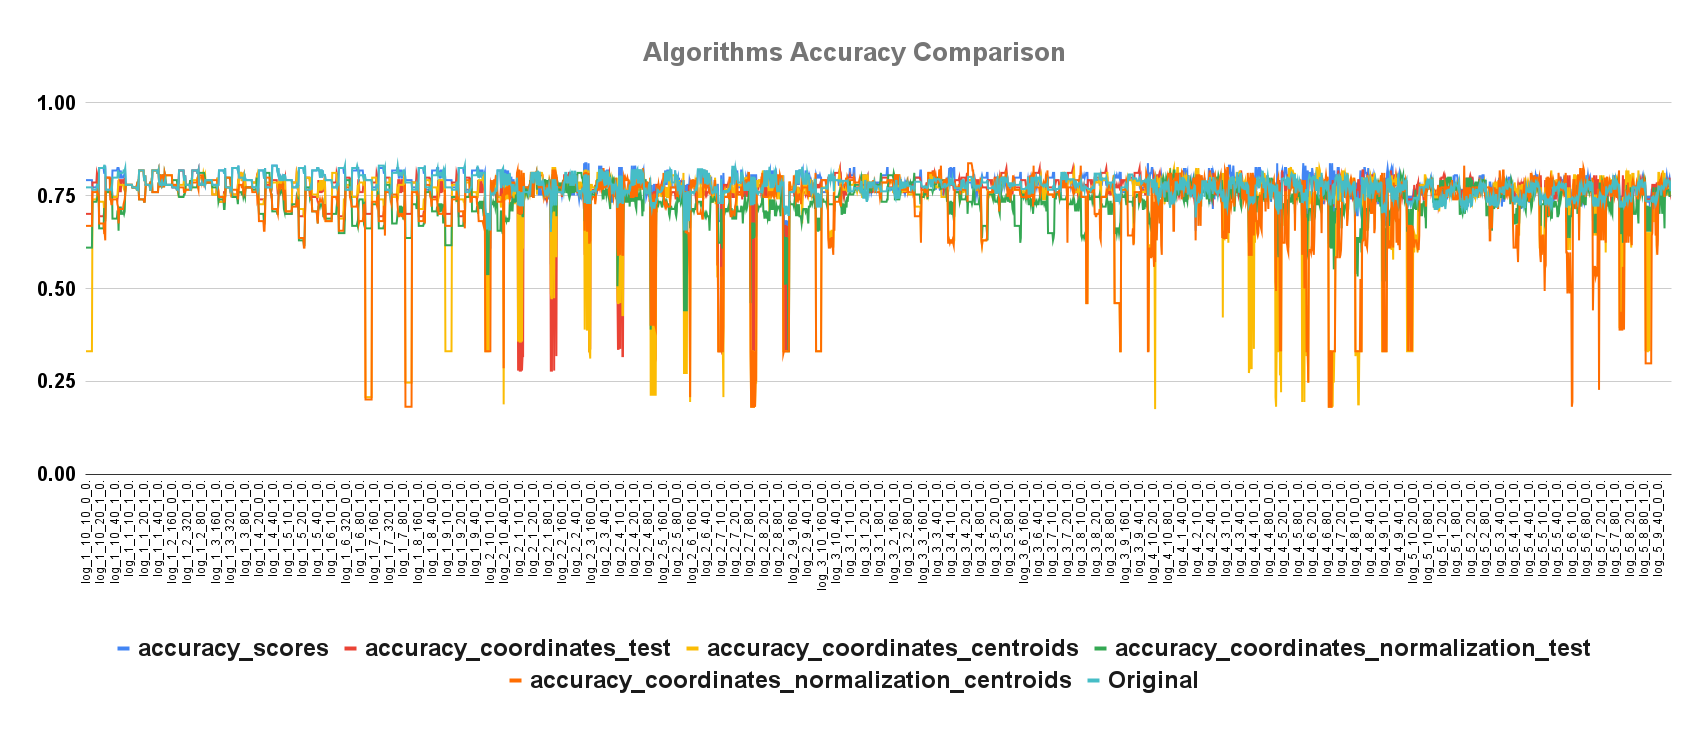
\includegraphics[width=\textwidth]{images/comparison_aggregation_algorithms1.png}
\caption{Comparison Between Aggregation Algorithms}
\label{fig:aggregation_comparison}
\end{figure}

For ease of reference, each algorithm is designated a numerical identifier as illustrated in Table 5.2.

\begin{table}[htbp]
\centering
\begin{tabular}{|c|c|}
\hline
Algorithm & Number \\
\hline
Only scores & 1 \\
\hline
Coordinates, distance to centroid & 2 \\
\hline
Coordinates, distance to test data & 3 \\
\hline
Normalized, distance to centroid & 4 \\
\hline
Normalized, distance to test data & 5 \\
\hline
\end{tabular}
\caption{Association Algorithm - Number}
\end{table}


Figure 5.1 offers a visual comparison of the inference accuracies of all algorithms. The y-axis represents accuracy while the x-axis details possible setting combinations, organized by ascending order based on the number of nodes, memory size, and number of neighbors. Remarkably, the simplest algorithm, algorithm 1, showcased commendable performance, even surpassing the original in specific settings. For configurations with four and five nodes, this algorithm's accuracy paralleled and occasionally outstripped, its more complex counterparts. In settings involving high memory size and five nodes, algorithm 5 stood out with 80\% accuracy in several instances, as opposed to about 70\% of the original one. Yet, algorithm 1 trailed by a mere 2\% and demonstrated greater consistency. The performance of algorithms 2 through 5 varied considerably with specific settings, ranging from an average of 79\% down to a nadir of 17.53\% for algorithm 2. Notably, algorithm 5 never dipped below 33\%. Algorithms 2 and 4, which gauged distances from centroids rather than test data, exhibited lackluster results, averaging a 3\% performance reduction. Their performance variability was also stark, plummeting to 17\% and 18\%, respectively, in contrast to their alternative techniques which maintained a floor of 28\% and 33\%. While algorithm 5 was projected to be the pinnacle of accuracy, its performance was hindered by unresolved issues in certain settings. For comprehensive details, the entire CSV file is accessible on the associated GitHub repository.


\newpage




